\chapter{Search by Snapのプロトタイプ}
\label{chapter:implement_sbs}
本章では,Search by Snapを用いて実装したプロトタイプについて述べる.

\section{システムの概要}
  \ref{section:design_sbs}節で述べたデザイン指針に基づき,\ref{chapter:implement_recog}章で用いた店舗を対象としたプロトタイプを実装する.
  OSM上では,飲食店などの店舗のオブジェクトは位置を定義された単一の点であるノードとして扱われ,各オブジェクトには``OSM ID''という一意の番号が付与されている.
  各店舗の看板画像とOSM IDを紐付け,Overpass API\footnote{http://overpass-api.de(2019/1/22確認)}を用いて店舗情報を取得する.これにより,\ref{chapter:implement_recog}章で実装したAPIを用いてリアルタイムで看板を認識し,店舗の看板から店舗情報へのアクセスができる.
  各店舗の店舗名とノードは表\ref{table:storename_to_osmid}に示す通り対応しており,表\ref{table:storelist}に示すそれぞれのノードには複数のタグが設定されている.
  ``name''は店舗の名称が代入されている.
  ``shop''タグは,店舗が販売している商品を記述するために使用される.
  飲食店の場合,施設の種類を表す``amenity''タグにバーやレストランのような店舗の種類が代入されている.
  ``opening\_hours''タグには,店舗の営業時間が代入されている.年中無休で24時間営業の場合は``24/7''が,曜日によって営業時間が異なる場合は,セミコロン区切りで複数の値が代入されている.例えば,小だるま JR高槻駅前店は,月曜日から木曜日までは11時30分から14時00分と17時から23時30分まで,金曜日,土曜日は11時30分から14時30分と17時00分から24時30分,日曜日は11時30分から23時30分が営業時間である.この場合,``opening\_hours''タグの値は
  ``Mo-Th 11:30--14:00, 17:00--23:30; Fr-Su 11:30--14:30, 17:00--24:30; Su 11:30--23:30''となる.
  支払いにクレジットカードが利用可能かどうかは,``american\_express'',``payment:diners\_club'',``payment:jcb'',``payment:master'',``payment:visa'',のタグに``yes''が代入されていれば利用可能である.表\ref{table:storelist}には``payment:visa''タグのみを掲載している.

  \begin{table}[tb]
    \caption{店舗名とOSM IDの対応}
    \label{table:storename_to_osmid}
    \begin{center}
      \begin{tabular}{c|c}
        \hline\hline
        \textbf{店舗名} & \textbf{OSM ID} \\ 
        \hline
        セブン-イレブン 高槻高槻町店 & 2391866925 \\
        全席個室居酒屋 北海の恩返し 高槻店 & 5279265335 \\
        小だるま JR高槻駅前店 & 5281672553 \\
        肉丼専門店 高槻肉劇場 & 5281672555 \\
        おだいどこはなれ 高槻店 & 5281672556 \\
        ビリヤード・ダーツ\&Food Bar Ozbuddy & 5281672557 \\
        磯丸水産 高槻店 & 5281672577 \\
        炭焼酒場 森田家 & 5281672578 \\
        メサベルテ 高槻店 & 5281672579 \\
        駿河屋 & 5281672580 \\
        甲南チケット 高槻本通店 & 5281672581 \\
        焼肉・しゃぶしゃぶ食べ放題 ぷくぷく 高槻店 & 5281672739 \\
        赤から 高槻店 & 5281672740 \\
        ちどり亭 高槻店 & 5281672835 \\
        高槻ちゃぶちゃぶ & 5281672942 \\
        \hline
      \end{tabular}
    \end{center}

    \caption{対象とする店舗のノード(2018年12月1日時点のOSMのデータベースを基に作成)}
    \label{table:storelist}
    \begin{center}
      \begin{tabular}{c|cccccc}
        \hline\hline
        \textbf{id} & \textbf{shop} & \textbf{amenity} & \textbf{opening\_hours} & \textbf{payment:visa} & \textbf{\ldots} \\ 
        \hline
        2391866925 & convenience & & 24/7 & yes & \\
        5279265335 & & bar & 17:00-24:00 & yes & \\
        5281672553 & & bar & Mo-Th 11:30-14:00; \ldots & yes & \\
        5281672555 & & restaurant & 11:00-23:00 & no & \\
        5281672556 & & bar & Mo-Th 11:30-24:00; \ldots & yes & \\
        5281672557 & & pub & Mo-Th 14:00-26:00; \ldots & no & \\
        5281672577 & & restaurant & 24/7 & yes & \\
        5281672578 & & restaurant & 17:00-26:00 & yes & \\
        5281672579 & bakery & & Mo-Sa 07:00-20:30; \ldots & no & \\
        5281672580 & hobby & & 10:00-23:00 & no & \\
        5281672581 & ticket & & Mo-Sa 10:00-19:00; \ldots & no & \\
        5281672739 & & restaurant & Mo-Fr 16:30-25:00; \ldots & yes & \\
        5281672740 & & bar & Mo-Fr 17:00-24:00; \ldots & yes & \\
        5281672835 & & restaurant & 17:00-25:00 & yes & \\
        5281672942 & & bar & 17:54-06:00 & yes & \\
        \hline
      \end{tabular}
    \end{center}


  \end{table}


\section{システムのインタフェース}
  クライアントサイドは,ユーザがOSを問わずに携帯端末で実行できるようにするために,HTML5とJavascriptを用いてWebアプリケーションとして実装した.
  インタフェースはデフォルトで端末の背面カメラ画面となっており,ユーザが前面カメラと切り替えられるようになっている.
  ユーザがカメラを通して店舗の看板を見ると,その店舗の店舗名,営業時間,使えるクレジットカードの種類などの情報が表示される.
  表示される店舗の種類や表示する情報の種類はユーザが選択できる.
  視覚情報の視認性を上げるために,減算型表示を用いてユーザにとって不要な情報は目立たなくすいる.
  Javascriptではカメラ映像をリアルタイムでの表示に十分な速度でグレースケール化できないため,不要部分に半透明の黒をマスクし,明度を下げることによって情報を減算している.
  実装したユーザインタフェースを図\ref{figure:sbs_interface}に示す.

\begin{figure}[tb]
  \centerline{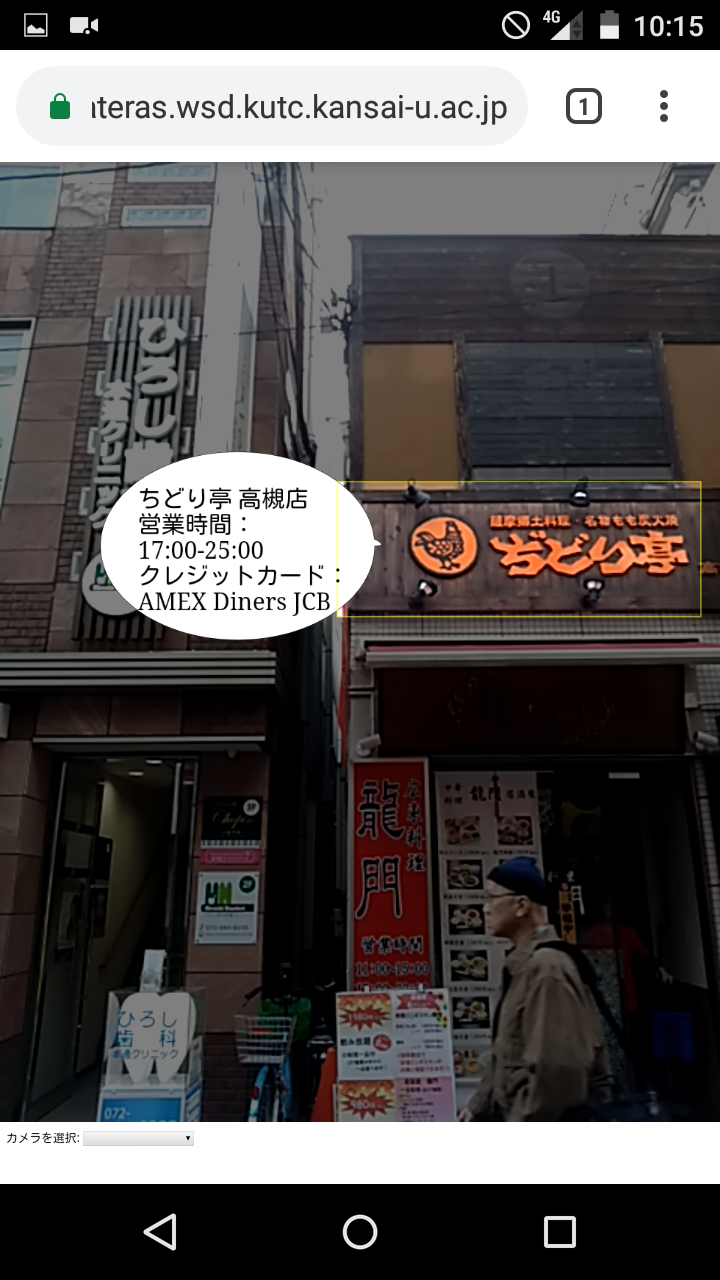
\includegraphics[width=.5\columnwidth, clip]{sbs_interface.png}}
  \caption{システムのインタフェース}
  \label{figure:sbs_interface}
\end{figure}

\section{システムの動作}
  提案システムにおいて,ユーザが取る行動とシステムが行う処理を以下に示し,図で表したものを図\ref{figure:sbs_system}に示す.
  \begin{enumerate}
    \item システムは携帯端末のGPS機能により,ユーザの位置情報を取得する
    \item ユーザは店舗の種類などのクエリを入力する
    \item システムはOverpass APIに位置情報とクエリを送信し,クエリに一致する周辺の店舗のOSM IDを取得する
    \item ユーザは携帯端末のカメラを通して街から画像情報を取得する(図\ref{figure:sbs_system}中\textcircled{\scriptsize 1})
    \item システムは画像をサーバに送信する(図\ref{figure:sbs_system}中\textcircled{\scriptsize 2})
    \item サーバはYOLOを用いて画像の中から看板領域を検出する(図\ref{figure:sbs_system}中\textcircled{\scriptsize 3})
    \item サーバは検出された看板領域を切り抜く(図\ref{figure:sbs_system}中\textcircled{\scriptsize 4})
    \item サーバはそれぞれの看板画像をVGG16を用いて店舗名でクラス分けする(図\ref{figure:sbs_system}中\textcircled{\scriptsize 5})
    \item サーバは画像内の看板の左上と右下の座標と検出した看板の店舗と関連付けられたOSMのノードのidをそれぞれ格納したJSONデータを生成する(図\ref{figure:sbs_system}中\textcircled{\scriptsize 6})
    \item サーバは生成されたJSONをシステムに返り値として返却する(図\ref{figure:sbs_system}中\textcircled{\scriptsize 7})
    \item システムはユーザが求めていない視覚情報の色調を低減させ,ユーザが求めている店舗の情報を看板の横に吹き出しとして重畳表示する(図\ref{figure:sbs_system}中\textcircled{\scriptsize 8})
    \item システムは認識した看板と関連付けられているOSM IDをOverpass APIに送信する(図\ref{figure:sbs_system}中\textcircled{\scriptsize 9})
    \item Overpass APIはOSM IDと一致する店舗のノードをシステムに返却する(図\ref{figure:sbs_system}中\textcircled{\scriptsize 10})
    \item システムは出力結果をユーザに提示する(図\ref{figure:sbs_system}中\textcircled{\scriptsize 11})
  \end{enumerate}

  \begin{figure}[tb]
    \centerline{\includegraphics[width=\columnwidth, clip]{sbs_system.pdf}}
    \caption{システムの動作}
    \label{figure:sbs_system}
  \end{figure}

  デバイスが画像をAPIに送信してからサーバがJSONデータを返却するまでに要した時間は,上り1Mbps,下り1.25Mbpsの通信速度,$980 \times 1307$の解像度で平均359msであった.
  Thropeらによると,人間が画面中央のオブジェクトを認識するまでのリアクションタイムの中央値は445msであるため\cite{Thorpe:1996},十分にユーザが満足できる速度であるといえる.
